\documentclass{article}
\usepackage[english]{babel}
\usepackage[a4paper,top=2.5cm,bottom=2cm,left=2.5cm,right=2.5cm,marginparwidth=1.75cm]{geometry}
\usepackage{amsmath}
\usepackage{graphicx}
\usepackage{subcaption} % For subfigures
\usepackage[colorlinks=true, allcolors=blue]{hyperref}
\usepackage{float}
\usepackage{titling}
\setlength{\droptitle}{-5em} 

\title{\textbf{Machine Learning: Exercise 1}}
\author{\textit{Amélie Assmayr (12007770)} \and
        \textit{Konstantinos Damanakis (12106343)} \and
        \textit{Teresa Schuch (12007762)}}
\date{}

\begin{document}
\maketitle
\vspace{-20pt}



\section{Introduction}
This report outlines the experimental design of the application of different classification algorithms across four diverse datasets. The goals is to show the trends in classifier performance, based on dataset properties like size and dimensionality, as well as the impact of preprocessing steps like scaling and different parameter settings.
The report is structured as followed: In Section 2 we introduce the chosen classifier and shortly explain their functionality. Section 3 describes the performance metrics used to evaluate each model across different configurations. Section 4 details the main characteristics of each datasets, the preprocessing steps applied and presents the evaluation results. Finally, in Section 5 discusses the main findings and insights drawn from the analysis.



\section{Classifiers}
We selected three distinct classifiers: an ensemble method (Random Forest), a margin-based method (SVM), and a distance-based method (KNN). This diverse selection will us help compare the effect of diffent classifiers better. Since we had a dataset where the target variable was non-binary we had to make sure to choose classifiers that can handle multiclass problems which is not the case for e.g. Logistic Regression.


\subsection{K-nearest-neighbors}
k-NN is a simple and intuitive classifier based on the proximity of instances. We wanted to see how it would handle the big datasets since it can be slow with large datsets. k-NN is also sensitive to the scale of the data, so it can help us identify the effect of scaling well. It works by finding the k training samples that are closest to the test sample, based on a distance metric and then making predictions based on the majority class of the neighbors.
In python there are several parameters that can be tuned to find the optimal result. These included:
\begin{itemize}
    \item \textbf{n\_neighbors:} \textit{k}
    \item \textbf{weights:} \textit{uniform} or \textit{distance}
    \item \textbf{Distance metrics:} \textit{Minkowski}, \textit{Eucildean} or \textit{Manhattan}
    \item \textbf{Algorithms:} \textit{ball\_tree}, \textit{kd\_tree} or \textit{brute}
\end{itemize}
\noindent \textit{n\_neighbors} specifies the number of nearest neighbors. Large values can help to smooth out outliers, but can also result in the lost of local patterns. 
\textit{weights} assigns weights to the neighbors. Uniform means that all neighbors have the same weight and therefore contribute equally, while with distance closer neighbors have a higher weight.
The distance evaluates the different distance metrics. Minkoswski distance is a generalization of the euclidean and manhattan distance and is given by 
\[
d(x, y) = \left( \sum_{i=1}^{n} |x_i - y_i|^p \right)^{\frac{1}{p}}
\]
To get the euclidean distance we can set p=2 and for the manhattan distance p=1.  The Chebyshev distance measures the maximum absolute difference along any dimension and is given by
\[
d(x, y) = \max_{i} |x_i - y_i|
\]


\subsection{Random Forest}
Random Forest (RF) is an ensemble method based on decision trees. Ensemble learning is based on the principle that a collectivity of learners achieves greater overall accuracy than a single learner. Therefore during learning the Random Forest algorithm constructs multiple decision trees and averages their prediction to yields more accurate and stable results. Each decision tree is trained only on a random subset of the training data obtained through bootstrapping. Furthermore for each split, only a randomly selected subset of features is considered. This reduces correlation between trees and enhances the generalization capability of the model. The most important hyperparameters in Random Forests include the number of trees (n\_estimators), the maximum depth of each tree (max\_depth), the minimum number of samples required to split a node (min\_samples\_split), and the minimum number of samples required to reach a leaf node (min\_samples\_leaf).
\\
We chose this algorithm because it can handle both numerical and categorical data well, making it a robust choice for our different datasets. Furthermore, random forests are robust to overfitting due to the averaging process over multiple trees. However, they can become computationally intensive when applied to very large data sets.


\subsection{Support Vector Machines}
Support Vector Machines (SVM) are supervised margin models that are based on finding the maximum-margin hyperplane that separates the classes. The optimal choice of hyperplane is the one that maximizes the distance (margin) from the support vectors (edge data points of each class). The higher the margin, the lower the generalization error of the classifier that is essential to avoid overfitting. The generalization error describes the the ability of the model to predict outcomes of new instances. The advantages of the SVM is its efficiency in high dimensional spaces and its versatility due to the use of kernels. On the other hand, the SVM is slow for large datasets and prone to overfitting if the number of features is much greater than the number of instances. In that case, a tuning of the parameters is critical.
\\
The Support Vector Machines use kernels, essentially mathematical functions that transform the data into a higher dimension. Typical kernel functions are "linear", "poly" (polynomial), "rbf" (radial basis function) or "sigmoid". Also, an important parameter is the regularization parameter (C) that is used to balance the maximization of the margin and the missclassification. High C decreases the margin and the missclassification while small C maximizes both. For the case of non-linear kernels (e.g rbf or poly), the parameter $\gamma$ is significant for the definition of decision boundary. Essentially, choosing a low gamma increases the influence of a training example on the nearby region of the feature space. On the other hand, a high gamma minimizes this influence, makes the decision boundary to be tight around individual points and as a result, favors the over-fitting.
\\
For the tests on the four datasets that are presented below, three different kernels have been tested, namely the linear, rbf and polynomial. The regularization parameter was set from the list [0.1, 1, 100, 1000], the hyperparameter $\gamma$ (only for non-linear kernels) was tuned according to the list [0.01, 1, 1000] and for the polynomial kernel degrees of 2,3 and 5 have been tested.
\newline
In the following sections, a few exemplary results from these classifiers will be shown.



\section{Performance Measures}
In order to ensure that the performance of the classifiers can be meaningfully compared, the following steps were taken:
\begin{itemize}
    \item \textbf{Dataset:} The same train/test splits were used across all classifiers to ensure consistency across all experiments. Furthermore the preprocessing (scaling, encoding, handling missing values) was the same for the datasets across the different classifiers.  
    \item \textbf{Parameter changes:} To compare how one hyperparameter affects the outcome, only a single hyperparameter was changed at a time. In the end the overall best combination.
    \item \textbf{Consistent performance measures:} We used the same set of performance measures for all our classifications.
\end{itemize}


\subsection{Training time}
Training time is important because larger or more complex models often give better results. However, it's important to check if the improvement is worth the additional training time. Especially with complex models and big datasets the time can increase exponentially when adding size, so looking for the time is very important.


\subsection{Accuracy}
$\text{Formula for binary target variables} = \frac{TP + TN}{TP + TN + FP + FN}$
Accuracy measures the proportion of correctly classified instances out of all instances. While it’s easy to interpret, it can be misleading, especially in imbalanced datasets, because it doesn't distinguish between false positives and false negatives.


\subsection{Precision}
$\text{Formula for binary target variables} = \frac{TP}{TP + FP}$
Precision measures how many of the positive predictions were actually correct and therefore measures the model’s ability to precisely identify relevant instances within the data. 
When we have multivariate target variable the presicion can be calculated by different ways In python you can choose between 'None (Class-Specific Metrics)', 'Macro Averaging', 'Micro Averaging' and 'Weighted  Averaging'. Let's assume that we have a target variable that has three categories:
With selection 'None' metrics are calculated for each class individually. That means that the precision would be calculated for each of the three classes and we would have three results. That is not always practical when you want to compare classifiers based on one metric.
For 'Macro' the metric is computed for each class individually and then the unweighted average is taken. For 'weighted average' the metric is also computed for each class indicidually, but each metric gets a wheigt based on the number of instances for this class. This can again be misleading when we have imbalaced data. 'Micro' focuses on overall performance instead of the individual classes.


\subsection{Recall}
$\text{Formula for binary target variable} = \frac{TP}{TP + FN}$
Recall measures how many true positive cases the model was able to identify. For multivariate target variables the same choice as in precision occurs.


\subsection{F1-score}
$\text{Formula}  = 2 \times \frac{\text{Precision} \times \text{Recall}}{\text{Precision} + \text{Recall}}$
The F1-score balances precision and recall. It thereby gives accurate results even if the dataset is skewed towards certain target classes. It might however be more difficult to immediately understand the score.



\section{Datasets}
We used four datasets to evaluate different classification methods. In addition to the \textit{Congressional Voting} and \textit{Amazon Reviews} datasets, which were given, we also selected the \textit{Machine Failure} and \textit{Road Traffic Accident} datasets. We ensured that all the datasets were diverse to assess how their different properties would affect the algorithms. \newline
First, the number of dimensions varies among the datasets. The \textit{Amazon Reviews} dataset has 750 instances and 10,002 variables, making it the dataset with the highest dimensionality. The dataset with the largest number of instances is the \textit{Road Traffic Accident} dataset, containing 12,290 instances and 32 variables. The \textit{Machine Failure} dataset includes 944 instances with 10 variables, while the smallest dataset is the \textit{Congressional Voting} dataset, with 218 samples and 18 dimensions.\newline
All the datasets, except for the \textit{Road Traffic Accident} dataset, have a binary target variable. The \textit{Road Traffic Accident} dataset has a multivariate target variable. Additionally, the \textit{Road Traffic Accident} and \textit{Congressional Voting} datasets contained missing values, necessitating preprocessing. The other two datasets had no missing values.\newline
More details about the datasets and their preprocessing are provided in their respective subsections.


\subsection{Congressional Voting}
This dataset contains the voting records of U.S. House of Representatives members. It has 18 columns and 218 observation, making it one of the smaller datasets used. It includes voting data on 16 key issues, where each vote is recorded as "Yes," "No," or "Unknown." The target variable indicates whether each representative is a Democrat or Republican. Additionally, there is an ID column for each representative. In Figure \ref{fig:plots_voting} the distribution of the target variable and the vote counts for each issue can be seen. It shows that the target variable is close to evenly balanced, with both categories having nearly the same number of instances. Furthermore it reveals that the dataset contains missing values (="Unknown") in each of the voting column which have to be handled as a preprocessing step.

\begin{figure}[H]
    \centering
    \begin{subfigure}[b]{0.45\textwidth}
        \centering
        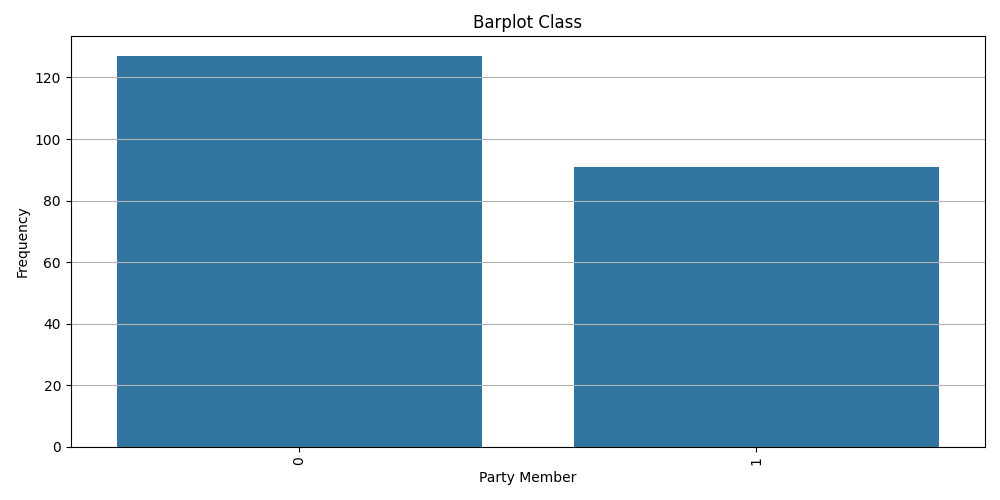
\includegraphics[width=\linewidth, height=5cm]{barplot_target_votings.png} 
        \caption{Barplot of target}
        \label{fig:figure1}
    \end{subfigure}
    \hspace{0.05\textwidth} % Adjust space between figures
    \begin{subfigure}[b]{0.45\textwidth}
        \centering
        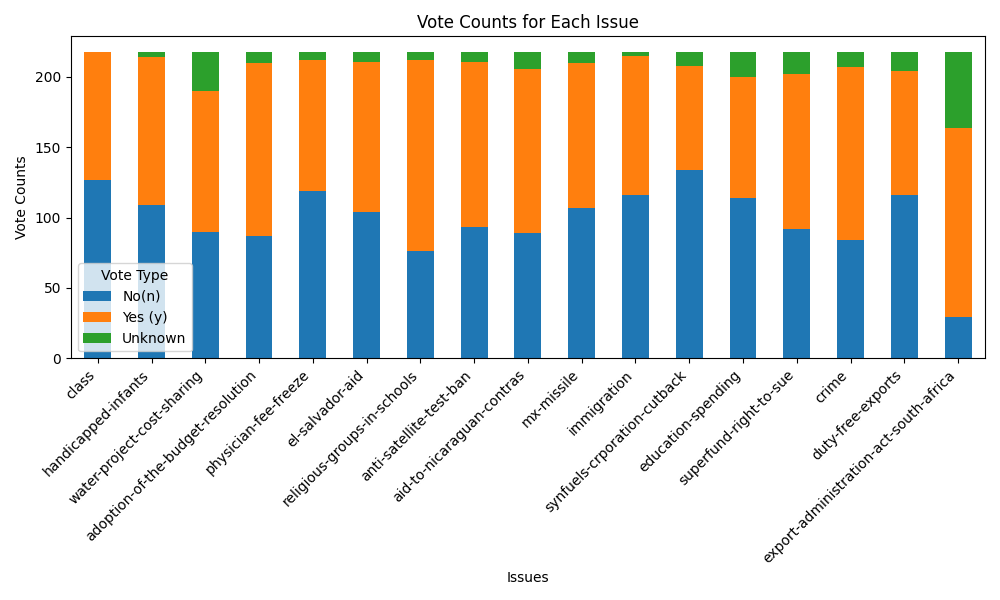
\includegraphics[width=\linewidth]{stacked_barplot.png} 
        \caption{Stacked Barplot votes}
        \label{fig:figure2}
    \end{subfigure}
    \caption{Plots - Congressional Voting}
    \label{fig:plots_voting}
\end{figure}


\subsubsection{Preprocessing}
First, a LabelEncoder is applied to convert the categorical variables into a binary format.  For the target variable, Democrats are encoded as 0s and Republicans as 1s.  In the vote columns, 'no' is encoded as 0s and 'yes' as 1s. Any 'unknown' values are replaced with NaN to mark them as missing. Next, rows with more than half of their values missing are removed from the dataset as they are considered to be too incomplete to provide useful information for analysis. The remaining missing values are then imputed by filling them with the most frequent value in each column. We decided to start with this straightforward method to see how well it works and decided to go back if we are unsatisfied with the results. Since the dataset consists only of binary data, there is no need for additional transformations like scaling or outlier handling. 


\subsubsection{Results}
\subsubsection*{k nearest neighbor}
We began our classification process by selecting k=3 as the starting value for K-Nearest Neighbors (KNN) and planned to adjust it later if needed. The baseline model already yielded excellent results, with all metrics exceeding 0.95. Cross-validation did not lead to improvements, likely because the model's performance was already near optimal. Scaling the data did not affect the results, as all the independent variables are binary. 
Next, we tried to adapt the parameters. We started by searching the optimal k. We set the range between 1 and 25, using accuracy as the deciding metric. The plot below illustrates the accuracy for different k values. The optimal weight was 'uniform', the optimal metric 'minkowski' and the optimal algorithm 'ball\_tree'.
Here are some of the times and performance measures.

\begin{table}[H]
\centering
\begin{tabular}{l|c|c|c|c|c|c}
\textbf{Model Parameters} & \textbf{Training Time (s)} & \textbf{Accuracy} & \textbf{Precision} & \textbf{Recall} & \textbf{F1} \\\hline
default (Holdout) & 0.0 & 0.9545 & 0.9524 & 0.9524 & 0.9524 \\
default (Cross-validated) & 0.1100  & 0.9242 & 0.8724 & 0.9524 & 0.9080\\
n=1 & 0.1016  & 0.9415 & 0.9042 & 0.9524 & 0.9256 \\
ball\_tree-algorithm & 0.1350  & 0.0.9474 & 0.9175 &0.9524 & 0.9317 \\
\end{tabular}
\caption{knn - Congressional Voting}
\label{tab:knn - Congressional Voting}
\end{table}

At the end we tried hypertuning our parameters. The hypertuning took approximately 12 seconds. The optimal parameters wehere 'ball\_tree' for the algorithms, 'minkowski' for the metric, k=2 and uniform weights. The accuracy was 0.9534, the precion = 0.9499, recall = 0.9534 and f1-score=0.9513.


\begin{figure}[H]
\centering
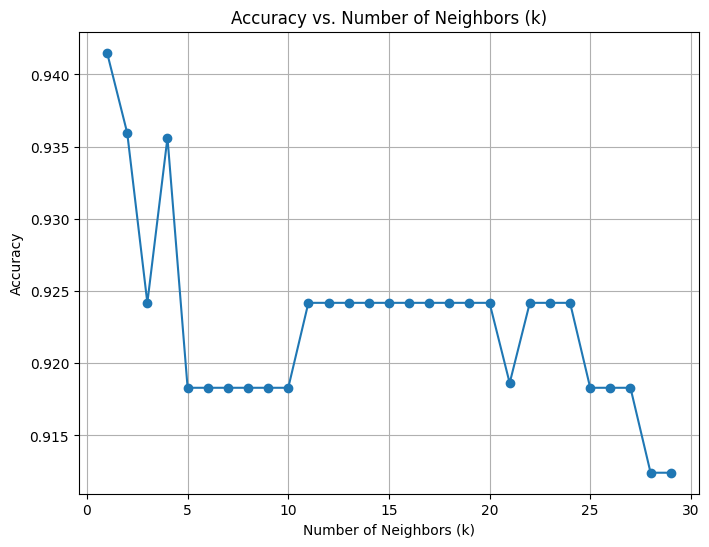
\includegraphics[width=0.8\linewidth]{voting_optimalK.png}
\caption{\label{fig:votingOptimalk} Correlation plot of some variables}
\end{figure}

\subsubsection*{Random forest}
The baseline Random Forest classifier has already very high performance across all metrics with scores consistently above 0.95, while also maintaining a very short training time. The 10-fold cross-validation gave slightly better scores, indicating a stable and reliable model across different splits. Therefore adjusting parameters yields only small changes in the results. In table \ref{table:Random Forest - Congressional Voting} the performance measures for some parameter changes are given. Increasing the parameter n\_estimators resulted in a noticeable increase in training time, while improving the metrics only slightly, emphasizing the importance of considering both performance and training time. Interestingly, hyperparameter tuning revealed that the best model was the one with the default parameter settings.

\begin{table}[H]
\centering
\begin{tabular}{l|c|c|c|c|c|c}
\textbf{Model Parameters} & \textbf{Training Time (s)} & \textbf{Accuracy} & \textbf{Precision} & \textbf{Recall} & \textbf{F1} \\\hline
default (Holdout) & 0.1851  & 0.9585 & 0.9545 & 0.9545 & 0.9545 \\
default (Cross-validated) & /  & 0.9634 & 0.9655 & 0.9634 & 0.9632 \\
n\_estimators=400 & 0.4508  & 0.9650 & 0.9698 & 0.9650  & 0.9646 \\
max\_depth=20 & 0.2089  & 0.9650 & 0.9698 & 0.9650 & 0.9646 \\
min\_samples\_leaf=10 & 0.1171  & 0.9598 & 0.9654 & 0.9598 & 0.9596 \\
min\_samples\_split=10 & 0.1127  & 0.9536 & 0.9625 & 0.9536 & 0.9536 \\
\end{tabular}
\caption{Random Forest - Congressional Voting}
\label{table:Random Forest - Congressional Voting}
\end{table}

Note that scaling is not applied to improve the performance of the Random Forest model for any of the datasets, as the algorithm is inherently scale-invariant.

\subsubsection*{Support Vector Machines}
The classification of the preprocessed dataset with Support Vector Machines gives very high metrics over a different range of hyperparameters, as it can be seen in Table \ref{table:votings_SVM}. Either linear, rbf or polynomial kernels achieve high performance. Also, the train times are very small for all of the kernels and parameter combinations. Efficiency and effectiveness are satisfied by SVM for this given dataset. This indicates that the preprocessed dataset has a clear structure. Therefore, there is no optimal kernel selection for this dataset, as high performance can be achieved with any of them, if the model is tuned to the optimal hyperparameters.
\begin{table}[h!]
\centering
\begin{tabular}{||c c c c c c c c c||} 
 \hline
 Kernel & C & $\gamma$ &d & Accuracy & Precision & Recall & F1 score & Train time [ms] \\ [0.5ex] 
 \hline\hline
 linear & 0.1 & - & - & 0.954 & 0.954 & 0.954 & 0.954 & 9 \\  
 rbf & 0.1 & 0.01 & - & 0.523 & 0.273 & 0.523 & 0.359 & 14 \\
 rbf & 1.0 & 0.01 & - & 0.977 & 0.978 & 0.977 & 0.977 & 12\\
 poly & 1.0 &  0.1 & 3 & 0.523 & 0.273 & 0.523 & 0.359 & 12 \\
 poly & 100 &  0.1 & 3 & 0.977 & 0.978 & 0.977 & 0.977 & 8 \\
 poly &  1.0&  1.0 & 5& 0.954 & 0.954 & 0.954 & 0.954 & 9 \\ [1ex] 
 \hline
\end{tabular}
\caption{Table including different used SVM parameters and the corresponding metrics.}
\label{table:votings_SVM}
\end{table}
\\
Among the parameters that were tested, the model has lower performance for non-linear kernels when the gamma hyperparameter is set too low. In particular, the model has a poorer performance for the rbf kernel, when the combination of $\gamma$ = 0.01 and C = 0.1 is used, and for poly kernel, when $\gamma$ = 0.1 and C $<$ 1.0. Using small $\gamma$, smoothens the decision boundary and oversimplifies the model that consequently for this given dataset, fails to classify correctly the different patterns. This is observed also for the rbf kernel, however when choosing C $\ge$ 1, due to the fact that the missclassifications are minimized, the performance of the model is improved in classifying the data. 
\\The processing time is negligible for all tested kernels and hyperparameters and since high accuracy and precision can be achieved with all kernels, the linear kernel would be chosen for this model due to its simplicity. The metrics for linear kernel do not change when different range of C parameter is chosen, therefore the model could be tuned to C=1.
\\Table \ref{table:votings_SVM_cross} shows a comparison of the metrics between the hold-out and the 10-fold cross-validation method, for linear kernel and C=1. A small improvement of effectiveness is observed with the cross-validation method that can be due to the fact that this method averages the performance over different splits.

\begin{table}[H]
\centering
\begin{tabular}{||c c c c c||} 
 \hline
Method &  Accuracy & Precision & Recall & F1 score \\ [0.5ex] 
 \hline\hline
hold-out & 0.954 & 0.954 & 0.954 & 0.954  \\  
 10-fold cross validation &  0.965&  0.968 & 0.965& 0.9659 \\ [1ex] 
 \hline
\end{tabular}
\caption{Table including comparison of metrics for hold-out nad 10-fold cross validation method, for linear kernel and C = 1.}
\label{table:votings_SVM_cross}
\end{table}


\subsection{Amazon Reviews}
The amazon reviews dataset includes 10002 columns and 740 rows. The large number of columns makes its classification quite challenging. Besides the, column 'ID' that includes the ascending number of row, there are 10000 columns that include an integer number between 0 and 32. The target variable ("Class") contains categorical data that are associated to names of famous authors such as "Bukowski", "Shea" etc. Although, the names of the columns do not clearly indicate what the integer values describe, it could be assumed that they represent the result of a counting.
\begin{figure}[H]
    \centering
    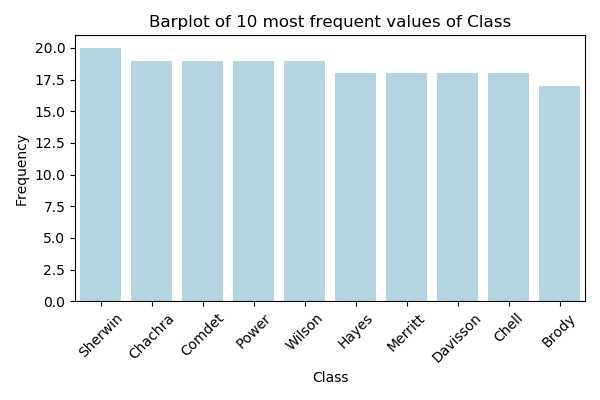
\includegraphics[width=.5\textwidth]{reviews_class.png}
    \caption{Barplot including 10 most frequent classes of output variable.}
    \label{fig:barplot_reviews}
\end{figure}
\begin{figure}[H]
    \centering
    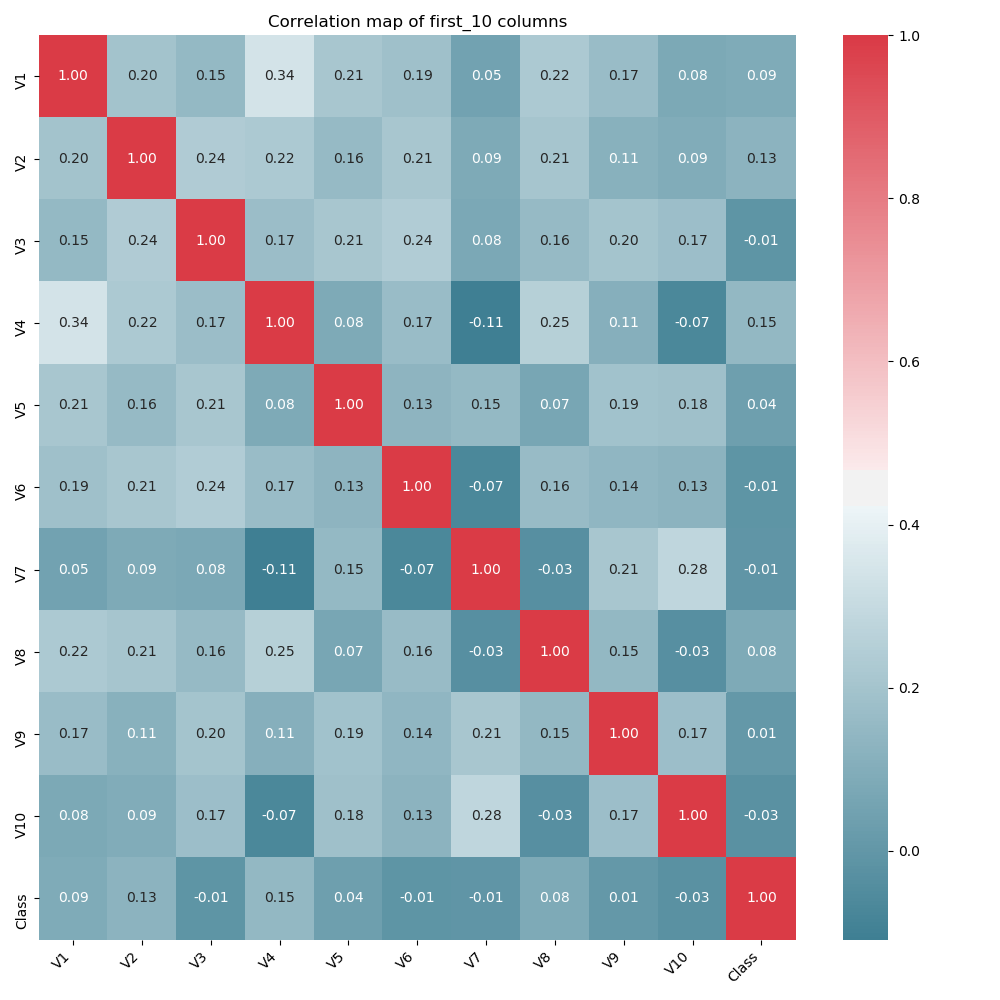
\includegraphics[width=.3\textwidth]{correlation_map_first_10.png}\hfill
    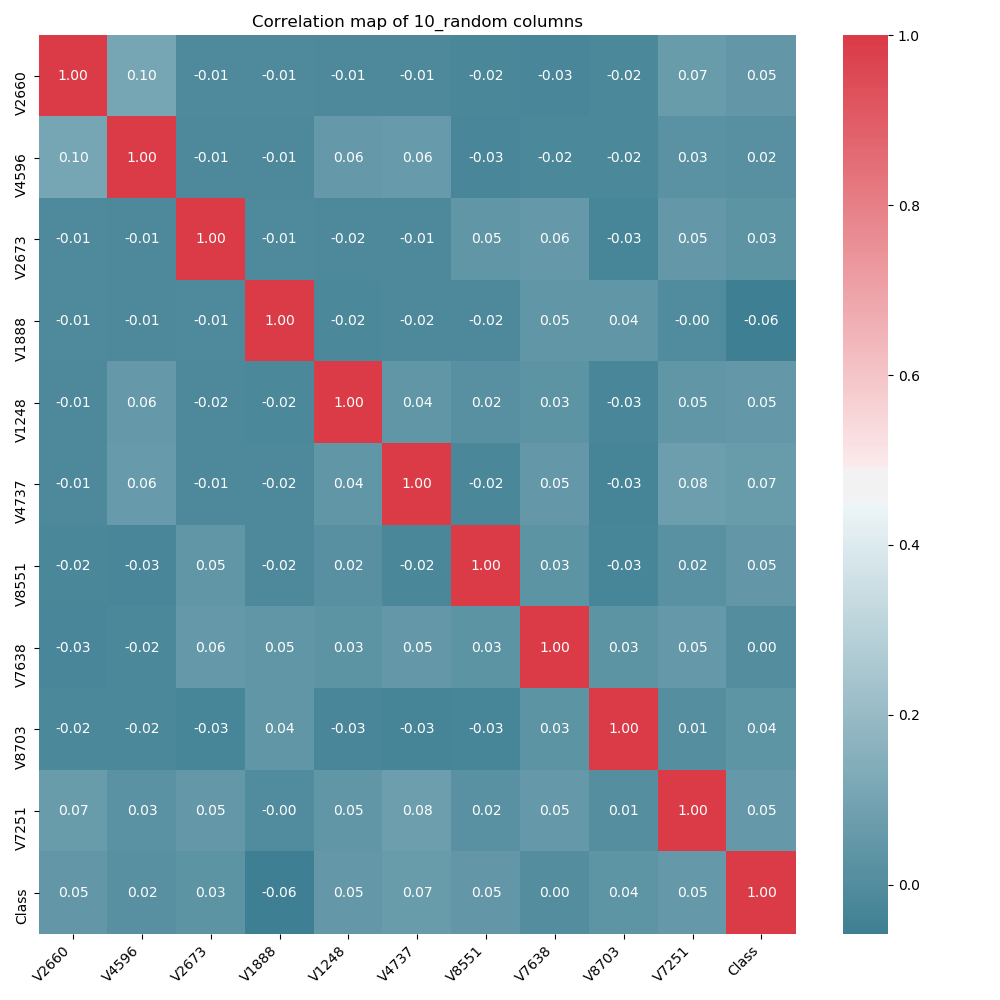
\includegraphics[width=.3\textwidth]{correlation_map_10_random.png}\hfill
    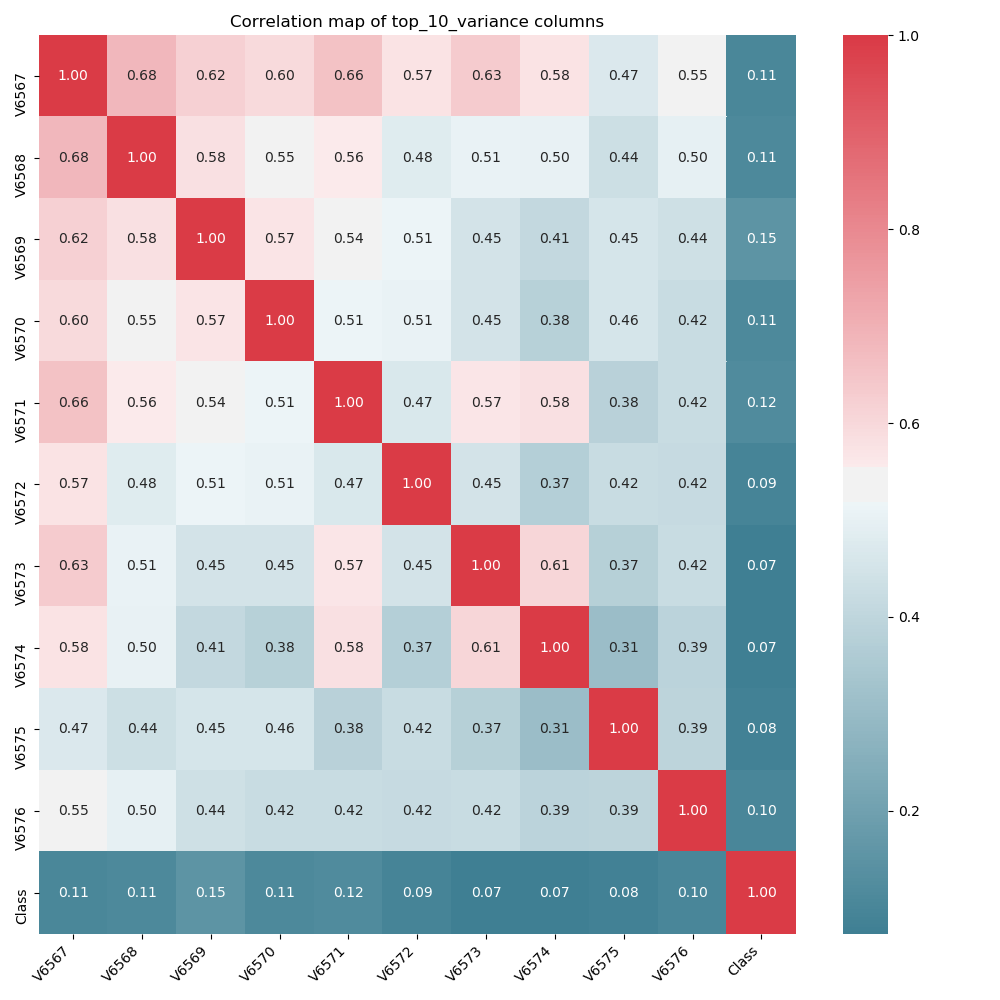
\includegraphics[width=.3\textwidth]{correlation_map_top_10_variance.png}
    \caption{Correlation plot including the class and first 10 columns (left), 10 random columns(middle), 10 columns with largest variance (right).}
    \label{fig:correlation_reviews}
\end{figure}


\subsubsection{Preprocessing}
Since all columns have integer types, except from the "Class", no encoding is necessary for the preprocessing of this dataset. The data neither feature any missing values nor any obvious outliers. Despite scaling of the data is not a necessary step, a standarization scaling is used.


\subsubsection{Results}
\subsubsection*{k nearest neighbor}
We began our classification process by selecting k=3 as the starting value for K-Nearest Neighbors (KNN) and planned to adjust it later if needed. Our baseline model was pretty bad with an accuracy of only 0.2. The weights precision was the highest performance parameter with also only a values of 0.4472. Scaling the data improved the weighted presicion parameter was worsend all the other which is why we continued with non-weighted data. The resaon why scaling might not have worked is because there weren't to many outliers in the data and a fixed range value. Cross validation also didn't improve our data. In this datset we had to use a 5-fold cross validation instead of a 10 fold since the datset was so small. 
We tried to find the optimal k in hopes to improve oour model. The optimal k for this model was 2. We could improve our accuracy slightly to 0.2300 in cross validation. We had two ides to improve the accury besides adapting the parameters. Namly dimension reduction and oversampling. 
We stared with dimensionality reduction. What worked best was removing coloms with correlation bigger then 0.9. We reduced features from 10000 to 8824. This already improved our accuracy slightly. Then we tried oversampling. This improved our accuracy  to 0.66 with 10 fold cross validation. Lastly we wanted to do hypertuning with our oversampled and reduced dataset to find out if it was even better.
Best parameters: {'algorithm': 'ball\_tree', 'metric': 'manhattan', 'n_neighbors': 4, 'weights': 'distance'}

\subsubsection*{Random forest}
The baseline Random Forest classifier achieves moderate performance, with an accuracy of 0.60. Compared to the votings dataset, the training time was significantly longer due to the large number of features and instances. The most notable improvement in terms of parameter settings came from increasing the n\_estimators parameter from 100 to 400. However this comes at the cost of very long training times of over 5 seconds. Another technique that worked very well was oversampling, which could achieve an accuracy of 0.78. Dimensionality reduction didn't improved the metrics. The best model from hyperparameter tuning is: \texttt{\{'min\_samples\_split': 5, 'n\_estimators': 400\}} which yields accuracy of 0.72. Table \ref{tab:Random Forest - Amazon Reviews} shows the performance metrics:

\begin{table}[H]
\centering
\begin{tabular}{l|c|c|c|c|c|c}
\textbf{Model Parameters} & \textbf{Training Time (s)} & \textbf{Accuracy} & \textbf{Precision} & \textbf{Recall} & \textbf{F1} \\\hline
default (Holdout) & 1.3971  & 0.6067 & 0.7017 & 0.6067 & 0.5817 \\
default (Cross-validated) & /  & 0.5933 & 0.7489 & 0.5933 & 0.5524 \\
oversampling (Cross-validated) & /  & 0.7870 & 0.8389 & 0.7870 & 0.7708 \\
dimension reduction (Cross-validated) & /  & 0.5587 & 0.7043 & 0.5587 & 0.5012 \\
n\_estimators=400 & 5.0367  & 0.6733 & 0.8146 & 0.6733 & 0.6154 \\
max\_depth=20 & 1.0564  & 0.5683 & 0.7553 & 0.5683 & 0.4920 \\
min\_samples\_leaf=10 & 0.4386  & 0.4367 & 0.7252 & 0.4367 & 0.3607 \\
min\_samples\_split=10 & 0.9904  & 0.5767 & 0.7561 & 0.5767 & 0.5148 \\
\end{tabular}
\caption{Random Forest - Amazon Reviews}
\label{tab:Random Forest - Amazon Reviews}
\end{table}


\subsubsection*{Support Vector Machines}
The metrics for the dataset as classified by Support Vector Machines over different model parameters (kernel function, C, gamma, degree of polynomial) are presented in table \ref{table:reviews_SVM}. The processing time is quite large for this dataset which is expected due to the large number of features and therefore, the complexity of the calculations. It is clear that effectiveness is relatively low for that classifier and dataset. Among the three different kernels, the linear shows the best performance in terms of performance. It is interesting that for a given kernel, tuning parameters such as C and $\gamma$ and using different ranges, seems to have no impact on the metrics. For the polynomial kernels, a second degree shows the highest metrics, however they are still very low. It should be noted that a standarization of the dataset has been performed before splitting the dataset. It is possible that the dataset includes a significant number of irrelevant features that apart from increasing the computing time, they impact and more precisely, saturate the accuracy when different hyperparameters are chosen. In that case, feature selection becomes an important step in order to optimize the performance of the model. 
\begin{table}[h!]
\centering
\begin{tabular}{||c c c c c c c c c||} 
 \hline
 Kernel & C & $\gamma$ &d & Accuracy & Precision & Recall & F1 score & Train time [ms]\\ [0.5ex] 
 \hline\hline
 linear & 1.0 & - & - & 0.606 & 0.704 & 0.606 & 0.611 &56049\\ 
 rbf & 100 & 0.01 & - & 0.013 & 0.0002 & 0.013 & 0.004 & 61713\\
 poly & 0.1 &  1.0 & 3 & 0.060 & 0.042 & 0.060 & 0.024 & 56398\\
 poly & 1.0 &  1.0&  2 & 0.073 & 0.055 & 0.733 & 0.039& 53921 \\ [1ex] 
 \hline
\end{tabular}
\caption{Table including different used SVM parameters and the corresponding metrics.}
\label{table:reviews_SVM}
\end{table}
\\
For the feature selection, the function SelectKBest of sklearn python library was used, and based on the F-value (describes the linear dependency of two parameters), the 100 first features were chosen. The processing time decreased substantially. For this subset and for linear kernel, the accuracy increased up to 0.646 and the precision up to 0.69. In addition, the train time reduced substantially, below 1 second. The metrics for the rbf kernel were unaffected while for the polynomial kernel were lower than before. The train time was about 560 ms for linear and about 1 s for rbf kernel. Repeating the same process and selecting the first 200 features, a further 5$\%$ increase is observed. However, in the ranges below 100 and above 200, the metrics follow a descending trend. This indicates that the optimal selection lies within the first 100 and 200 features, if this approach for feature selection is followed. In any case, only a small optimization is possible with this method. More sophisticated optimization methods for feature selection would be necessary in order to achieve higher performance.
\\
It should be noted that when the scaling of data is skipped in preprocessing, the metrics deteriorate, with the accuracy dropping to 0.5. This is expected for Support Vector Machines because the algorithm relies on calculating distances between the data for determining the decision boundary, and primarily, the support vectors. 
\\ 
The table \ref{table:reviews_SVM_cross} compares the acquired metrics between hold-out and 10-fold cross-validation method. For this dataset, the hold-out method gives better metrics than the 10-fold cross validation. This indicates that the split set given by the hold-out method might not fully represent the complexity of relationships within the dataset. 
\begin{table}[h!]
\centering
\begin{tabular}{||c c c c c||} 
 \hline
Method &  Accuracy & Precision & Recall & F1 score \\ [0.5ex] 
 \hline\hline
hold-out & 0.606 & 0.704 & 0.606 & 0.611  \\  
 10-fold cross validation &  0.560&  0.506 & 0.560& 0.501 \\ [1ex] 
 \hline
\end{tabular}
\caption{Table including comparison of metrics for hold-out and 10-fold cross validation method, for linear kernel and C = 1.}
\label{table:reviews_SVM_cross}
\end{table}


\subsection{Road Traffic Accidents}
The \textit{Road Traffic Accident} dataset contains records of road traffic accidents that occurred between 2017 and 2020 in Addis Ababa, Ethiopia. This dataset provides detailed information about the severity of accidents, the number and characteristics of the involved vehicles and individuals, the areas where the accidents occurred, and other relevant factors.
We selected this dataset because it addresses a critical public safety issue. Analyzing this data can help predict the severity of road accidents, which may, in turn, identify key causes and factors contributing to road safety. Additionally, this analysis could be valuable for stakeholders such as insurance companies and car rental services by providing insights into accident risks based on factors like the driver, vehicle type, timing, and location.
\newline
Missing data can be observed in 16 of the 32 features. Overall there are s 20.057 missing values. In the following table all attributes, their datatype(r=ratio quantity, o=ordinal, n=nominal), the number of unique elements for categorical variables and the number of missing values can be seen :
\setlength{\tabcolsep}{1pt} % Reduce padding in table cells
\begin{table}[H]
    \parbox{.5\linewidth}{
        \begin{tabular}{l@{}c@{}c@{}c}
            \textit{\textbf{Variable}} & \textbf{Type} \hspace{0.3em} & \textbf{Unique} \hspace{0.3em} & \textbf{Missing}\\\hline
            \textit{Time} & r & / & / \\
            \textit{Day of Week} & n & 7 & /\\
            \textit{Age of Driver} & o & / & /\\
            \textit{Sex of Driver} & n & 3 &/ \\
            \textit{Educational Level} & n & 7 & 741\\
            \textit{Vehicle-Driver Relation} & n & 4 & 579 \\
            \textit{Driving Experience} & o & / & 829\\
            \textit{Vehicle Type} & n & 17 & 950\\
            \textit{Vehicle Owner} & n & 4 & 482\\
            \textit{Vehicle Service Year} & r & / & 3928\\
            \textit{Defect of Vehicle} & n & 3 & 4427\\
            \textit{Accident Area} & n & 14 & 239\\
            \textit{Lanes or Medians} & n & 7 & 385\\
            \textit{Road Alignment} & n & 9 & 142\\
            \textit{Junction Type} & n & 8 & 887\\
            \textit{Road Surface Type} & n  & 4 & 172
        \end{tabular}
    }
    \hfill
    \parbox{.5\linewidth}{
        \begin{tabular}{l@{}r@{}c@{}c}
            \textit{\textbf{Variable}} & \textbf{Type} \hspace{0.3em} & \textbf{Unique} \hspace{0.3em} & \textbf{Missing}\\\hline
            \textit{Road Surface Condition} & n & 4 & 172\\
            \textit{Light Condition} & n & 4 & /\\
            \textit{Weather Condition} & n & 9 &/\\
            \textit{Collision Type} & n & 10  & 155\\
            \textit{Number of Vehicles} & r & / &/\\
            \textit{Number of Casualty} & r & / &/\\
            \textit{Vehicle Movement} & n & 13 & 308\\
            \textit{Casualty Class} & n & 4 &/ \\
            \textit{Sex of Casualty} & n & 3 & / \\
            \textit{Age of Casualty} & r & / & /\\
            \textit{Casualty Severity} & o & 4 & / \\
            \textit{Work of Casualty} & n & 7 & 3198\\
            \textit{Fitness of Casualty} & n & 5 & 2635 \\
            \textit{Pedestrian Movement} & n & 9 &/ \\
            \textit{Cause of Accident} & n & 20 & /\\
            \textit{Severity of Accident} & n & 3 & /
        \end{tabular}}
\end{table}


\subsubsection{Preprocessing}
When reading in the data, all variables were initially imported as character variables, so we first converted them to their appropriate types. All numeric variables were converted to numeric, ordinal variables were transformed into ordered factors, and the time variable was converted into a time format. Additionally, all variables containing values such as "NA," "", "NULL," "unknown," "Unknown," or "na" were treated as missing values. To simplify handling, the hour was extracted from the \textit{Time} variable, as it originally had many unique values.
We started our preprocessing by calculating the correlation of your variables.\newline
We began our preprocessing by calculating the correlation between variables. For numeric and ordered variables, we used Spearman correlation, while for other variables, we calculated Cramér's V. Due to the large number of variables, it is impractical to show a correlation plot for all of them. Instead, the correlation of the numeric and ordered variables is presented in Figure \ref{fig:cor_RTA}:
\begin{figure}[H]
\centering
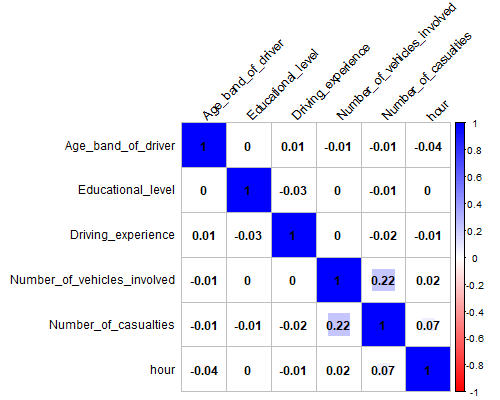
\includegraphics[width=0.8\linewidth]{plots_correlation_num_RTA.png}
\caption{\label{fig:cor_RTA} Correlation plot of some variables}
\end{figure}
As shown in Figure \ref{fig:cor_RTA}, \textit{Number of Casualties} and \textit{Number of Vehicles Involved} have a small correlation. Additionally, \textit{Area Accident Occurred} and \textit{Owner of Vehicle}, as well as \textit{Road Alignment} and \textit{Area Accident Occurred}, exhibit small correlations. Conversely, \textit{Weather Conditions} and \textit{Road Surface Conditions}, as well as \textit{Pedestrian Movement} and \textit{Casualty Class}, have high correlations.
Next, I addressed missing values. Rows with more than one-third of their values missing were removed, resulting in the deletion of 26 rows, which had no significant impact. Columns with more than half of their values missing were also removed. Furthermore, the \textit{Time} variable was excluded since it was replaced by the \textit{Hour} variable. Notably, many recorded times ended in "0" or "5" (e.g., 12:00 and 12:05) compared to times like 12:04, indicating that time values were often rounded.
Finally, I removed the following variables due to high percentages of missing values and limited relevance to the question or their lack of correlation with \textit{Accident Severity}: \textit{Age Band of Casualty}, \textit{Casualty Severity}, \textit{Work of Casualty}, and \textit{Fitness of Casualty}.
\newline
To impute the missing values, we applied different approaches based on the nature of the variables and the amount of missing data. The variables \textit{Sex of Driver}, \textit{Vehicle Driver Relation}, \textit{Owner of Vehicle}, \textit{Area Accident Occurred}, \textit{Lanes or Medians}, \textit{Road Alignment}, \textit{Road Surface Type}, \textit{Type of Collision}, \textit{Vehicle Movement}, and \textit{Cause of Accident} were imputed using their mode. This approach was chosen because these variables had relatively few missing values and no strong correlations with other variables.
For \textit{Type of Junction}, \textit{Educational Level}, and \textit{Age Band of Driver}, the missing values were imputed using proportional allocation to reflect the original distribution of the data.
For variables with higher correlations, we used imputation based on related variables. For example, \textit{Weather Conditions} was imputed based on \textit{Road Surface Conditions}. If \textit{Road Surface Conditions} was "Snow," \textit{Weather Conditions} was imputed as "Snow." If \textit{Road Surface Conditions} was "Flood over 3cm deep" or "Wet or Damp," \textit{Weather Conditions} was imputed as "Raining," and for other cases, it was imputed as "Normal." Similarly, missing values in \textit{Casualty Class} were imputed based on \textit{Pedestrian Movement}, and missing values in \textit{Educational Level} were imputed based on \textit{Vehicle Driver Relation}.


\subsubsection{Target variable}
The target variable is \textit{Severity of Accident}, which is categorized into three classes: \textit{Slight Injury}, \textit{Serious Injury}, and \textit{Fatal Injury}. While the severity could technically be considered an ordinal variable, we treated it as nominal and framed the task as a multiclass classification problem.
The following plot shows the distribution of these classes. It is evident that the classes are unevenly distributed. Most accidents fall under the \textit{Slight Injury} category, followed by \textit{Serious Injury}, while only a small number of accidents are classified as \textit{Fatal Injury}. This class imbalance is a critical consideration, and methods such as bootstrapping or oversampling could be employed to address it effectively.

\begin{figure}[H]
\centering
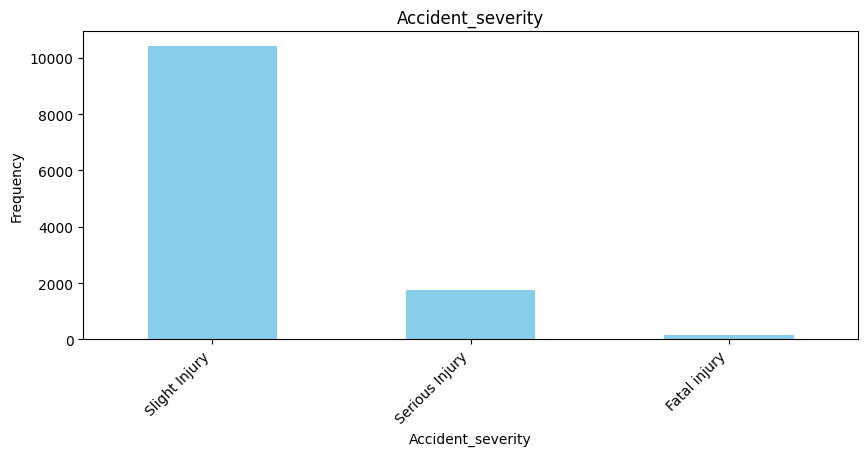
\includegraphics[width=1\linewidth]{Accident_severity.png}
\caption{\label{fig:bar:severity} Barplot of Accident Severity}
\end{figure}



\subsubsection{Results}
\subsubsection*{Random forest}
For the Road Traffic Accidents dataset, the default Random Forest classifier performed well, achieving an accuracy of 0.85. Modifying the parameters resulted in little to no improvement. Also the best model from hyperparameter tuning yield accuracy 0.85 with parameter: \texttt{\{'max\_depth': 20, 'n\_estimators': 200\}}. However, applying oversampling significantly boosted the performance, leading to near-perfect scores of 0.99 across all metrics.


\begin{table}[H]
\centering
\begin{tabular}{l|c|c|c|c|c|c}
\textbf{Model Parameters} & \textbf{Training Time (s)} & \textbf{Accuracy} & \textbf{Precision} & \textbf{Recall} & \textbf{F1} \\\hline
default (Holdout) & 0.9436  & 0.8596 & 0.8461 & 0.8596 & 0.8004 \\
default (Cross-validated) & /  & 0.8469 & 0.8009 & 0.8469 & 0.7813 \\
oversampling (Cross-validated) & /  & 0.9964 & 0.9965 & 0.9964 & 0.9964 \\
n\_estimators=400 & 4.3679  & 0.8471 & 0.8032 & 0.8471  & 0.7812 \\
max\_depth=20 & 0.9068  & 0.8477 & 0.8272 & 0.8477 & 0.7815 \\
min\_samples\_leaf=10 & 0.7349  & 0.8455  & 0.8694 & 0.8455 & 0.7747 \\
min\_samples\_split=10 & 0.9158  & 0.8468 & 0.8152 & 0.8468 & 0.7791 \\
\end{tabular}
\caption{Random Forest - Road Traffic Accidents}
\label{tab:Random Forest - Road Traffic Accidents}
\end{table}


\subsubsection*{Support Vector Machines}
The metrics in Table \ref{table:rta_SVM} show that for either linear, rbf or poly kernels a high precision and accuracy is achieved when the model is tuned to specific parameter combinations. The best performance parameters per kernel show saturated metrics. An interpation could be that the dataset is linear separable, therefore linear kernels perform well enough and trying more complex kernels such as the non-linear ones, does not lead to any improvement of the metrics. The train time is relatively large for all of the kernels shown in \ref{table:rta_SVM}. For the linear kernels, selecting C$>$1 increases significantly the processing time (in the order of several minutes), rendering the computational cost not optimal. For rbf and poly kernels, a wider range of the hyperparameter C can be tested within a meaningful processing time, only when gamma is set low, such as $\gamma$ = 0.01 or vice-verca, a wider range of gamma can be tested only when C is chosen to be small (e.g C $\le$1). Larger values of $\gamma$ and C increase computational time, with the former forcing the model to define a decision boundary more tight around individual points, as mentioned in section \ref{svm}, and the latter leads to stricter fitting of the data. 
\\ 
Therefore, the road traffic accident dataset requires simpler decision boundaries which means that C and $\gamma$ should be chosen to be small. Regarding the kernel selection, any of the tested shows same performance, therefore a linear kernel could be the choice due to its simplicity.  
\begin{table}[h!]
\centering
\begin{tabular}{||c c c c c c c c c||} 
 \hline
 Kernel & C & $\gamma$ &d & Accuracy & Precision & Recall & F1 score & Train time [ms] \\ [0.5ex] 
 \hline\hline
 linear &  1.0 & - & - & 0.857 & 0.734 & 0.857 & 0.790 & 5095 \\
  rbf &  1.0 & 0.01 & - & 0.857 & 0.734 & 0.857 & 0.790 & 18852\\
 poly &  0.1 & 0.01 & 3 & 0.857 & 0.734 & 0.857 & 0.790 & 5751 \\[1ex] 
 \hline
\end{tabular}
\caption{Table including different used SVM parameters and the corresponding metrics.}
\label{table:rta_SVM}
\end{table}
\\
Table \ref{table:rta_SVM_cross} shows the comparison of the metrics between the hold-out and the 10-fold cross-validation method, for linear kernel and C=1. The metrics are very similar for both methods. This shows that the split of the dataset with the hold-out method results in a quite representative subset of the whole, that gives similar results with the averaging that is performed by cross-validation method.
\begin{table}[h!]
\centering
\begin{tabular}{||c c c c c||} 
 \hline
Method &  Accuracy & Precision & Recall & F1 score \\ [0.5ex] 
 \hline\hline
hold-out & 0.856 & 0.734 & 0.856 & 0.790  \\  
 10-fold cross validation &  0.842&  0.710 & 0.842& 0.770 \\ [1ex] 
 \hline
\end{tabular}
\caption{Table including comparison of metrics for hold-out nad 10-fold cross validation method, for linear kernel and C = 1.}
\label{table:rta_SVM_cross}
\end{table}


\subsection{Machine Failure}
The \textit{Machine Failure} dataset contains sensor data collected from various machines, including a range of sensor readings and records of machine failures. The primary goal of this dataset is to predict whether a machine will fail or not.
We selected this dataset because it addresses an important issue in industrial settings. Unexpected machine failures can result in significant financial losses for companies. Predicting potential failures in advance allows for timely maintenance and replacement, ensuring operational efficiency and reducing downtime.
\noindent There are no missing values in this dataset. The following table lists all the attributes, their data types (\textit{r} = ratio quantity, \textit{o} = ordinal, \textit{n} = nominal), and the number of unique elements:
\setlength{\tabcolsep}{1pt} % Reduce padding in table cells
    \begin{table}[H]
        \begin{tabular}{l@{}c@{}c@{}c}
                \textit{\textbf{Variable}} & \textbf{Type} \hspace{0.3em} & \textbf{Unique} \hspace{0.3em} \\\hline
                \textit{footfall } & r & 99 \\
                \textit{tempMode} & r & 8 \\
                \textit{AQ} & r & 7 \\
                \textit{USS} & r & 7 \\
                \textit{CS} & r & 7 \\
                \textit{VOC} & r & 7  \\
                \textit{RP} & r & 71 \\
                \textit{IP} & r & 7 \\
                \textit{Temperature} & r & 24 \\
                \textit{fail} & r & 2 
        \end{tabular}
    \end{table}

While the data types in the \textit{Road Traffic Accident} were divers with mainly charcter variables here we have only numeric variables. All the variables are integers.


\subsubsection{Preprocessing}
Since there were no missing values preprocessing was not really necessary, but we did look at the correlation of the variables to see if some might be redundant. We used the pearson correlation. AS we can see the dataset has some high correlations especially beween \textit{VOC} and \textit{fail} and between \textit{VOC} and \textit{AQ}. In this dataset approximately 58,36\% of machines are not failing and 41, 63\% are .So this variable is approximately uniformly distributed. 
\begin{figure}[H]
\centering
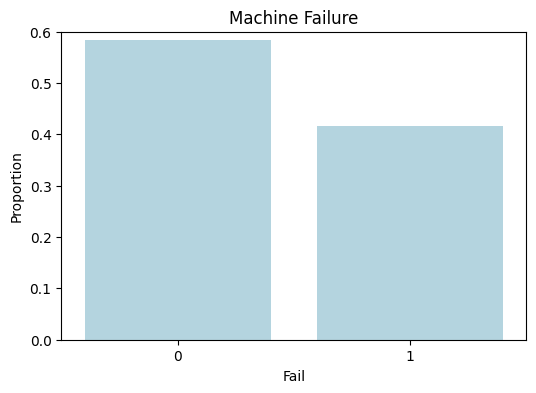
\includegraphics[width=1\linewidth]{MachineFailure.png}
\caption{\label{fig:bar:failure} Barplot of Machine Failure}
\end{figure}
\begin{figure}[H]
\centering
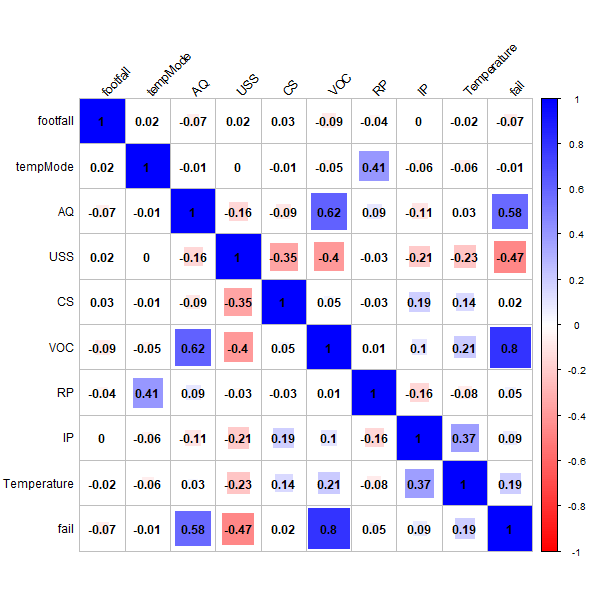
\includegraphics[width=0.8\linewidth]{plots_correlation_Machine.png}
\caption{\label{fig:cor_machine} Correlation plot}
\end{figure}


\subsubsection{Results}
\subsection*{k nearest neighbor}
Our baseline model already gave us pretty good accuracy. All performance measures were around between 0.74 and 0.79. Here we were hopeful that scaling would help since we only had numeric independent variables. We were right since our accuracy increased to 0.85 with an houldout model and to 0.912 with 10 fold cross validation. Then we tried to find optimal parameters and always changed on at the time before doing hypertuning. Here are the performance measure for some experiments:

\begin{table}[H]
\centering
\begin{tabular}{l|c|c|c|c|c|c}
\textbf{Model Parameters} & \textbf{Training Time (s)} & \textbf{Accuracy} & \textbf{Precision} & \textbf{Recall} & \textbf{F1} \\\hline
default (Holdout) & 0.0020 & 0.8571 & 0.8409 & 0.8506 & 0.8457 \\
default (Cross-validated) & 0.1245  & 0.9126 & 0.8862 &0.9022 & 0.8934\\
n=17 & 0.1234  & 0.9206 & 0.8951 & 0.9118 & 0.9031 \\
minkowski-algorithm & 0.1293  & 0.9206 & 0.8951 & 0.9118 & 0.9031 \\
\end{tabular}
\caption{knn - Machine Failure}
\label{tab:knn - Machine Failure}
\end{table}

Hyperparameter tuning (finding best parameter combinations):
Best parameters: {'algorithm': 'ball_tree', 'metric': 'manhattan', 'n_neighbors': 23, 'weights': 'uniform'}
Best cross-validation accuracy: 0.9232
Best cross-validation precision: 0.9247
Best cross-validation recall: 0.9232
Best cross-validation F1 Score: 0.9234
Time for Hypertuning:  11.81977128982544

\subsubsection*{Random forest}
The default Random Forest classifier for the Machine Failure dataset achieved an accuracy of 0.88, which is already satisfactory. Adjusting the parameter settings did not result in significant performance changes. However, adjusting the min\_samples\_leaf parameter to 10 led to the greatest improvement, increasing the accuracy to 0.90 without affecting the training time. The best hyperparameters found through tuning were \texttt{{'min\_samples\_leaf': 5, 'n\_estimators': 400}}, which also resulted in an accuracy of 0.90. The performance metrics are shown below:

\begin{table}[H]
\centering
\begin{tabular}{l|c|c|c|c|c|c}
\textbf{Model Parameters} & \textbf{Training Time (s)} & \textbf{Accuracy} & \textbf{Precision} & \textbf{Recall} & \textbf{F1} \\\hline
default (Holdout) & 0.1463  & 0.8836 & 0.8840 & 0.8836 & 0.8837 \\
default (Cross-validated) & /  & 0.8772 & 0.8870 & 0.8772 & 0.8749 \\
n\_estimators=400 & 0.6035  & 0.8846 & 0.8933 & 0.8846  & 0.8827 \\
max\_depth=20 & 0.1553  & 0.8772 & 0.8870 & 0.8772 & 0.8749 \\
min\_samples\_leaf=10 & 0.1373  & 0.9035  & 0.9075 & 0.9035  & 0.9037 \\
min\_samples\_split=10 & 0.1460  & 0.8792 & 0.8904 & 0.8792 & 0.8777 \\
\end{tabular}
\caption{Random Forest - Machine Failure}
\label{tab:Random Forest - Machine Failure}
\end{table}


\subsubsection*{Support Vector Machines}
Table \ref{table:machine_SVM} shows some exemplary results for different combinations of input hyperparameters. All three kernels give high accuracy and precision if the parameters are tuned carefully. A selection of linear kernel gives high metrics for different ranges of C. For rbf kernel, choosing $\gamma$=0.01 for different C parameters gives a good precision and accuracy but this is not the case for larger $\gamma$. Processing time is small for most of the combinations, however as gamma grows beyond 0.01, the accuracy and precision deteriorate and classification seems to be more prone to overfitting. Regarding the polynomial kernel and degree$=$3, the accuracy is high for most of the tested parameters, except from low $\gamma$ and C. Effectiveness decreases with $\gamma$ which is an indication of underfitting. In general, this different behavior when varying the kernel implies some complexity within the dataset. Nevertheless, for every kernel, the hyperparameters can be tuned accordingly in order to achieve high metrics. Linear kernel performs better in terms of efficiency and training time.
\begin{table}[h!]
\centering
\begin{tabular}{||c c c c c c c c c||} 
 \hline
 Kernel & C & $\gamma$ &d & Accuracy & Precision & Recall & F1 score & Train time [ms] \\ [0.5ex] 
 \hline\hline
 linear & 0.1 & - & - & 0.878 & 0.878 & 0.878 & 0.878 & 31 \\
 linear & 100 & - & - & 0.883 & 0.883 & 0.883 & 0.883 & 1066 \\
 rbf & 0.1 & 0.01 &- &  0.888 & 0.888 & 0.888 & 0.888 & 120  \\
 rbf & 0.1 & 1.0 & - & 0.539 & 0.291 & 0.539 & 0.378 & 197 \\
 poly & 0.1 &  1.0 &  3 & 0.878 & 0.880 &  0.878 & 0.878 & 142  \\ 
 poly & 1.0 &  0.01 &  3 & 0.540 & 0.291 &  0.540 & 0.378 & 75  \\[1ex] 
 \hline
\end{tabular}
\caption{Table including different used SVM parameters and the corresponding metrics.}
\label{table:machine_SVM}
\end{table}
\\ 
Table \ref{table:machine_SVM_cross} shows the comparison of the metrics between the hold-out and the 10-fold cross-validation method, for linear kernel and C=1. The metrics estimated after the 10-fold cross-validation method is used are slightly higher, in the order of 5$\%$, in comparison to the hold-out method. 
\begin{table}[h!]
\centering
\begin{tabular}{||c c c c c||} 
 \hline
Method &  Accuracy & Precision & Recall & F1 score \\ [0.5ex] 
 \hline\hline
hold-out & 0.883 & 0.883 & 0.883 & 0.883  \\  
 10-fold cross validation &  0.915&  0.916 & 0.915& 0.915 \\ [1ex] 
 \hline
\end{tabular}
\caption{Table including comparison of metrics for hold-out nad 10-fold cross validation method, for linear kernel and C = 1.}
\label{table:machine_SVM_cross}
\end{table}

\section{Discussion of Findings}
In Table \ref{tab:model_performance} we can see the best result in terms of F1 for each dataset×classifier pair.

\begin{table}[H]
\centering
\begin{tabular}{l|c|c|c}
\hline
\textbf{Dataset}       & \textbf{KNN} & \textbf{RF} & \textbf{SVM} \\ \hline
Congressional Voting & 0.9646 & xxx & xxx \\ 
Amazon Reviews  & 0.7708 & xxx & xxx \\ 
Road Traffic Accidents & 0.9964 & xxx & xxx \\ 
Machine Failure & 0.9037 & xxx & xxx \\ \hline
\end{tabular}
\caption{Performance metrics (F1 score) of different models across datasets.}
\label{tab:model_performance}
\end{table}



\section{Notes}

\end{document}